\pdfoutput=1
\documentclass[11pt]{article}

% Change "review" to "final" for the camera-ready; "preprint" for arXiv.
\usepackage[review]{acl}

\usepackage{times}
\usepackage{latexsym}
\usepackage[T1]{fontenc}
\usepackage[utf8]{inputenc}
\usepackage{graphicx}
\usepackage{booktabs}
\usepackage{multirow}
\usepackage{array}
\usepackage{colortbl}
\usepackage{amsmath}
\usepackage{pifont}
\usepackage{url}
\newcommand{\cmark}{\ding{51}}
\newcommand{\xmark}{\ding{55}}
\definecolor{guidanceblue}{RGB}{222,235,247}
\newcommand{\gcell}[1]{\cellcolor{guidanceblue}#1}
\newcommand{\gbox}[1]{\begingroup\setlength{\fboxsep}{1.2pt}\colorbox{guidanceblue}{\strut #1}\endgroup}
% hyperref is loaded by acl.sty; do not load it here (avoids option clash).

\title{WorkSurface-Bench: Benchmarking Enterprise Agents on\\
Multi-Surface Knowledge Routing}

\author{Anonymous ARR submission}

\begin{document}
\maketitle

\begin{figure*}[t]
\centering
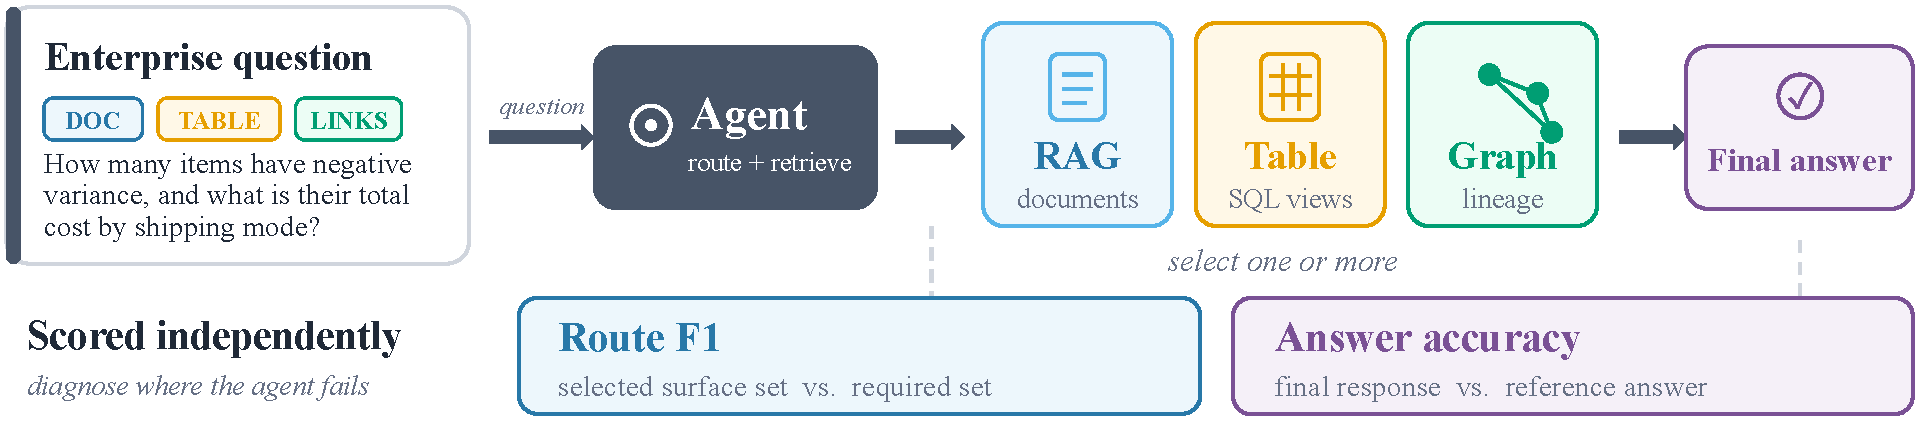
\includegraphics[width=0.98\textwidth]{figure1_teaser_polished.pdf}
\caption{WorkSurface-Bench projects a shared enterprise benchmark corpus onto three
canonical surfaces (RAG, Table, Graph) and scores \emph{Route} (surface
selection) and \emph{Answer} (final correctness) as separate metrics.}
\label{fig:teaser}
\end{figure*}

\begin{abstract}
Enterprise agents often need several kinds of knowledge at once: documents
for narrative facts, tables for calculations, and dependency graphs for file
relationships. Existing benchmarks usually test retrieval or tool use, but do
not separate \emph{choosing the right knowledge form} from using it correctly.
We introduce \textbf{WorkSurface-Bench}, which evaluates this choice as
\emph{surface routing}. The benchmark projects five persona-scoped
Workspace-Bench-Lite workspaces onto document, table, and graph surfaces and
contains 1{,}151 atomic tasks. Its reference answers are auditable: table answers
come from executed DuckDB queries, document answers are checked against
verbatim spans, and graph answers derive from source annotations. We evaluate
four backbones under five agent settings, yielding 23{,}020 retained
trajectories with no protocol errors. Gold-surface guidance raises Route F1 to 98.7--99.8, yet Answer
reaches only 50.2--64.1\%. Cross-surface Answer peaks at 45.7\%, below every
single-surface category. In an independent three-annotator audit, all 200
sampled tasks pass all six criteria by majority vote. We release the
construction pipeline, scoring code, and agent harness at
\url{https://github.com/haolpku/WorkSurface-Bench}.
\end{abstract}

\section{Introduction}
\label{sec:intro}

Consider an operations analyst asking: \emph{``Which source files feed the
negative-variance inventory report, and what is the total logistics cost by
shipping mode?''} The agent must read a report for context, query a table for
the total, and follow a dependency graph to identify the source files. These
are not interchangeable operations. Document retrieval cannot perform a SQL
aggregate, and a table query does not reveal file lineage. Before answering,
the agent must first decide which kinds of knowledge the question requires.

We call each kind of knowledge a \emph{surface}. In this paper, \textbf{surface
routing} means selecting the document, table, or graph surfaces needed for a
question. This capability is usually hidden inside an end-to-end score. RAG
benchmarks \citep{friel2024ragbench,chen2020hybridqa,chen2021ottqa} mainly ask
whether the final answer is correct. If a model chooses the wrong source or
retrieves the wrong evidence, both failures simply produce an incorrect
answer. Tool-use benchmarks
\citep{huang2023metatool,chen2023teval,li2023apibank} evaluate API selection,
but they do not test whether an agent recognizes that a question requires a
different representation of knowledge, such as SQL rather than prose search.
For deployment, this distinction matters: choosing the right surface and
reasoning correctly after that choice are separate abilities.

We introduce \textbf{WorkSurface-Bench} (Figure~\ref{fig:teaser}) to measure
both abilities. We project five persona-scoped workspaces onto three routable
surfaces: a document knowledge base, a DuckDB table registry, and a file
dependency graph. Procedural SOPs remain task metadata rather than a fourth
routable surface. Each task receives four scores---Route, Evidence, Answer,
and Efficiency---so the evaluation shows whether an agent chose the right
surface, found the right evidence, answered correctly, and used a reasonable
amount of computation. Reference answers never come directly from model free
text: we execute table queries, verify document spans, and derive graph answers
from source annotations.

This separation makes failures easier to interpret. A low Route score means
the agent chose the wrong surfaces; a low Evidence score means it chose the
right surfaces but did not find the required items. If Route and Evidence are
high but Answer is low, the remaining problem is computation or synthesis.
End-to-end accuracy alone cannot distinguish these cases.

We evaluate four backbones (GPT-4o-mini, DeepSeek-V4-Pro, Gemini-3.1-Pro, and
GPT-5.5) under five agent settings on 1{,}151 tasks. The main
result is simple: \textbf{better routing does not guarantee a better answer}.
Gold-surface guidance raises Route F1 to 98.7--99.8, while Answer remains at
50.2--64.1\%. Cross-surface Answer peaks at only 45.7\%. Even after an agent
knows where to look, it can still retrieve the
wrong evidence, combine sources incorrectly, or make a computation error.

Our contributions are:
\begin{enumerate}
\item \textbf{A multi-surface routing benchmark}
(\S\ref{sec:dataset}): 1{,}151 tasks from five persona-scoped workspaces, projected
onto document, table, and graph surfaces. To our knowledge, it is the first
workspace benchmark to score surface routing separately from the Answer metric.
\item \textbf{A verifiable construction pipeline}
(\S\ref{sec:derivation}): deterministic rules and verified LLM-assisted
proposals produce gold answers from executed queries, checked spans, or source
graph annotations rather than model-generated values.
\item \textbf{A diagnostic scoring protocol} (\S\ref{sec:scoring}): Route,
Evidence, Answer, and Efficiency are scored separately, making it possible to
locate failures that one end-to-end score would hide.
\item \textbf{Evidence that routing and answering differ}
(\S\ref{sec:experiments}): gold-surface guidance improves Route F1 much more
than Answer across four complete backbone sweeps with no retained protocol errors.
\end{enumerate}

\section{Related Work}
\label{sec:related}

% ---- inlined from table_prior.tex ----
% Table 1: prior-benchmark comparison (paper_spec §3.6)
\begin{table*}[t]
\centering
\small
\resizebox{\textwidth}{!}{%
\begin{tabular}{lccccc}
\toprule
\textbf{Benchmark} & \textbf{\#Surfaces} & \textbf{Route metric} & \textbf{Enterprise src} & \textbf{Skill/SOP} & \textbf{Graph type} \\
\midrule
Workspace-Bench 1.0 & files (1 form) & \xmark & \cmark & rubric & file-dep (1-hop) \\
STaRK & 2 (text+KG) & \xmark & \xmark & \xmark & concept KG \\
HybridQA & 2 (text+table) & \xmark & \xmark & \xmark & --- \\
OTT-QA & 2 (text+table) & \xmark & \xmark & \xmark & --- \\
T\textsuperscript{2}-RAGBench & 2 (text+table) & \xmark & \xmark & \xmark & --- \\
MMQA & 3 (text+table+image) & \xmark & \xmark & \xmark & --- \\
MetaTool & tools (100s) & \cmark\,(tool) & \xmark & \xmark & --- \\
T-Eval & tools & \cmark\,(step) & \xmark & \xmark & --- \\
API-Bank & APIs ($\sim$50) & \cmark\,(API) & \xmark & \xmark & --- \\
RAGBench & 1 (docs) & \xmark & partial & \xmark & --- \\
BIRD / Spider & 1 (SQL) & \xmark & \xmark & \xmark & --- \\
TheAgentCompany & env (tools+web) & \xmark & \cmark & \xmark & --- \\
\midrule
\textbf{WorkSurface-Bench (ours)} & \textbf{3 routable + SOP metadata} & \cmark\,(surface) & \cmark & \cmark\,(SOP) & file lineage+enrich \\
\bottomrule
\end{tabular}%
}
\caption{Positioning against prior benchmarks. WorkSurface-Bench projects
three routable knowledge surfaces over a shared enterprise corpus, attaches
SOP metadata, and scores surface routing separately from answer correctness.
Entries are based on the cited benchmark descriptions.}
\label{tab:prior}
\end{table*}
% ---- end table_prior.tex ----

WorkSurface-Bench sits at the intersection of four active benchmark
threads: multi-source retrieval-augmented QA, enterprise-scale agent
evaluation, tool and API routing, and semi-structured knowledge retrieval.
Table~\ref{tab:prior} places representative benchmarks along the two axes we
care about --- how many categorically distinct \emph{surfaces} are present,
and whether surface selection itself is a scored metric --- and shows that
the combination is not represented among the surveyed benchmarks.

\subsection{Multi-source Retrieval-Augmented QA}
The earliest attempts to move beyond single-surface RAG fused \emph{two}
sources into one integrated question. HybridQA \citep{chen2020hybridqa} pairs
Wikipedia tables with linked passages; OTT-QA \citep{chen2021ottqa} extends
this to 400K open-domain tables and 5M passages; T$^2$-RAGBench
\citep{isgorur2026t2ragbench} adds financial text-and-table retrieval; and
MMQA \citep{talmor2021mmqa} combines text, tables, and images. In all of
these, the answer requires evidence from both surfaces, but the model is
never asked to \emph{decide} whether it needs the table or the text --- both
are simply retrieved. Recent benchmarks broaden the retrieval target
(RAGBench~\citep{friel2024ragbench} standardises RAG evaluation, and BIRD /
Spider \citep{li2023bird,yu2018spider} isolate text-to-SQL), but they still operate over
a single surface. WorkSurface-Bench adds a third routable surface, a
dependency graph, and makes the selection decision itself a first-class
score.

\subsection{Semi-structured Knowledge Retrieval}
STaRK \citep{wu2024stark} evaluates retrieval over semi-structured knowledge
bases where a concept-level knowledge graph (entities, typed relations)
is blended with textual descriptions. Our Graph surface is different in kind:
it encodes \emph{workspace-native file lineage} (file-depends-on-file,
file-supports-output, task-requires-file), not concept-level ontology
relations. File lineage is the graph a real enterprise agent must reason
over --- ``which spreadsheets feed this dashboard?'' is a graph traversal
that no KG-QA benchmark captures. Prior work on KG-augmented retrieval
therefore complements rather than duplicates our Graph surface.

\subsection{Tool and API Routing}
A parallel line of work \emph{does} score routing explicitly, but at a
different granularity: MetaTool \citep{huang2023metatool} tests whether a
model chooses among $\sim$200 tools; T-Eval \citep{chen2023teval} decomposes
tool use into instruct/plan/reason/retrieve/understand/review steps;
API-Bank \citep{li2023apibank} evaluates $\sim$50 REST APIs. In all cases
the choice space is a large flat catalogue of \emph{homogeneous} operational
endpoints (add\_event, search\_web, translate, \ldots). Our surfaces are
distinct \emph{information types}, not distinct operations --- there are
only three of them, and the decision is qualitatively different from
picking one API out of two hundred. Tools are the operational vehicle;
surfaces are the information type.

\subsection{Enterprise Workspace Agents}
Workspace-Bench \citep{tang2026workspacebench} evaluates whether agents can
produce workspace deliverables end-to-end over hundreds of files with rich
dependencies; TheAgentCompany \citep{xu2024theagentcompany} evaluates agents
in a broader enterprise environment (web, tools, colleague chat) on
consequential tasks. Both target end-to-end deliverable success ---
``did the agent produce the report?'' --- and both are complementary to our
question, ``which knowledge form should the agent have consulted?''.
WorkSurface-Bench inherits Workspace-Bench's source data and provenance
pipeline but shifts the evaluation target from workspace \emph{learning} to
workspace \emph{routing}, and enriches the one-hop file dependency graph
into a graph surface that supports multi-hop lineage queries.

\section{Benchmark Construction}
\label{sec:dataset}

WorkSurface-Bench is built by a deterministic pipeline that adds no synthetic
facts, followed by a verifiable LLM-assisted expansion. Figure~\ref{fig:pipeline}
gives the overview; we detail each stage below and report the resulting
statistics in Table~\ref{tab:stats}.

\begin{figure*}[t]
\centering
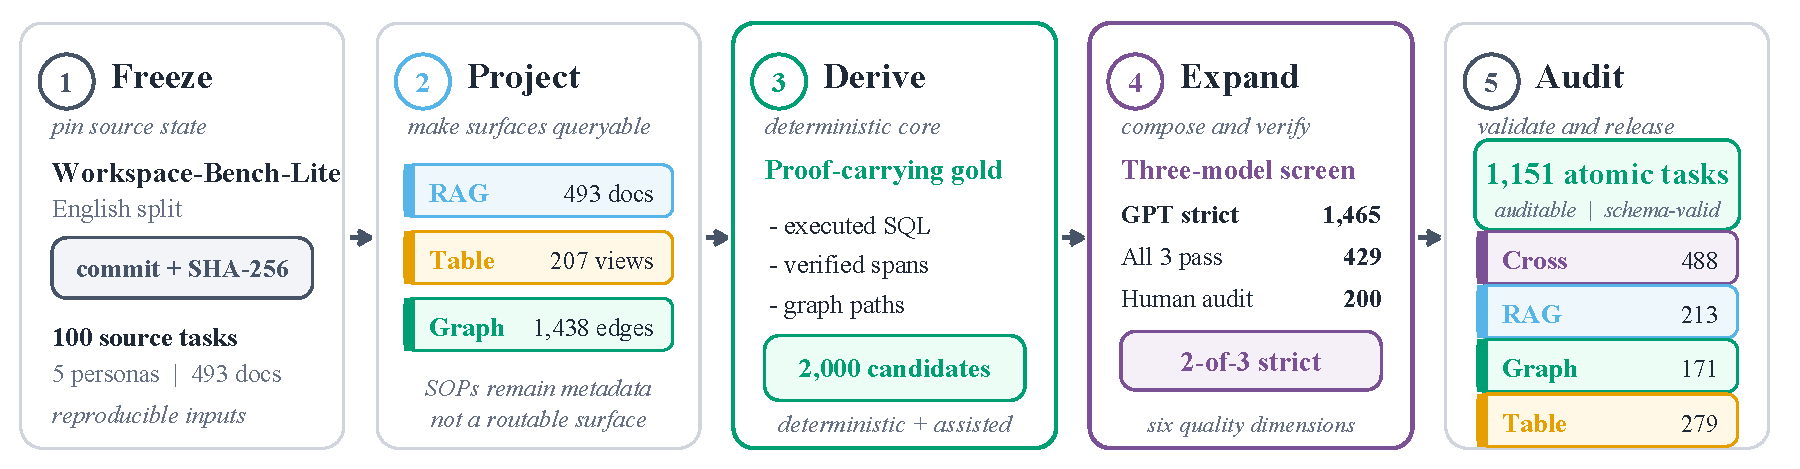
\includegraphics[width=0.98\textwidth]{figure2_pipeline.pdf}
\caption{Construction pipeline. Gold answers trace to executed DuckDB results,
verified document spans, or source dependency annotations; no gold value is
taken from model free text. Details in \S\ref{sec:derivation}.}
\label{fig:pipeline}
\end{figure*}

% ---- inlined from table_stats.tex ----
\begin{table}[t]
\centering
\small
\begin{tabular}{lr}
\toprule
\textbf{Statistic} & \textbf{Value} \\
\midrule
Personas & 5 \\
Source tasks (WSB-Lite) & 100 \\
Atomic tasks & 1{,}151 \\
\quad cross\_surface & 488 \\
\quad rag\_only & 213 \\
\quad graph\_only & 171 \\
\quad table\_only & 279 \\
Persona count range & 39--595 \\
Routable surfaces & 3 \\
KB canonical docs & 493 \\
Table views (DuckDB) & 207 \\
Graph edges (total) & 1{,}438 \\
Executed table-bearing gold & 453/453 \\
RAG-bearing span verification & 601/601 \\
Graph-bearing path verification & 600/600 \\
2-of-3 screening pass & 1{,}151/2{,}000 \\
Efficiency budgets & 1{,}151/1{,}151 \\
\bottomrule
\end{tabular}
\caption{WorkSurface-Bench statistics. Every table-bearing gold is an executed
DuckDB query result; RAG-bearing evidence is verified against document spans,
and graph golds derive from source dependency annotations
(\S\ref{sec:derivation}).}
\label{tab:stats}
\end{table}
% ---- end table_stats.tex ----

\subsection{Source Data and Provenance}
\label{sec:provenance}
We derive the benchmark from the Workspace-Bench-Lite English split. Its data
pipeline is hybrid: task scenarios and dependency graphs are human-authored and
expert-validated from real Lark/ByteDance workflows, while file contents
combine public web resources with grounded LLM-generated artifacts. We do not
claim ``real enterprise data''; we claim enterprise-scenario-grounded hybrid
data with human-authored task/rubric/graph annotations. The first pipeline
stage freezes the source commit and every input file's SHA-256 in a lock file,
and evaluate closed-book answerability separately
(\S\ref{sec:closedbook}).

\subsection{Surface Projection}
\label{sec:surfaces}
Each persona workspace is projected onto three routable surfaces.
\textbf{RAG}: documents, reports, PDFs, and slide text are converted to
canonical UTF-8 markdown so routing is evaluated separately from OCR/parsing.
\textbf{Table}: a per-workbook DuckDB view registry over normalized CSV/XLSX,
with provenance columns; a coverage gate keeps only non-trivial sheets as
tables and demotes the rest to RAG. \textbf{Graph}: the Workspace-Bench file
dependency graph enriched with programmatic edges (\texttt{mentions},
\texttt{schema\_overlap}, \texttt{version\_of}, \texttt{shared\_artifact}).
SOPs derived from repeated rubric patterns are attached as
\texttt{applicable\_skills} metadata; in this release they are not a routable surface,
because a rubric promoted verbatim leaks its task's answer. Each surface passes
executable eligibility and leakage checks reported in
Appendix~\ref{sec:appendix}.

\subsection{Task Derivation}
\label{sec:derivation}
Atomic tasks are derived in two passes. The \emph{deterministic} pass adds no
synthesized facts: numeric rubric values ($\$$1{,}710{,}971.47, 16.89\%,
``1000 records'') are extracted as gold answers; a \texttt{graph\_only} task
per source task asks which files are required inputs; and \texttt{cross\_surface}
tasks are emitted only when a DuckDB aggregate over a \emph{named} column
reproduces the rubric's figure, so the gold query is semantically valid rather
than a numeric coincidence. The \emph{verifiable LLM-assisted} pass reaches
target scale without trusting model free-text: for table and cross-surface
tasks the model proposes a DuckDB query that we execute (gold $=$ the result),
and for RAG tasks it proposes a question whose answer we verify occurs verbatim
in the source document. Items whose query errors or whose answer is absent are
dropped. Graph-only golds are derived directly from source dependency
annotations. A final QC pass deduplicates and re-validates against the schema.

\subsection{Automatic Validation and Model-assisted Screening}
\label{sec:qc}

We generate a 2{,}000-item candidate pool and first apply deterministic schema,
uniqueness, language, leakage, query-execution, span, and graph-path checks.
Every table-bearing item must reproduce its gold through a read-only query,
every RAG-bearing item must point to a verified span, and every graph-bearing
item must match a source dependency path. IDs and normalized questions must
also be unique.

We then apply a semantic screen for answerability, gold correctness,
naturalness, atomicity and unambiguity, necessity of the declared surfaces,
and absence of leakage cues. GPT-5.5 retains 1{,}465 candidates under this
strict rubric. Independent DeepSeek and Gemini audits produce the final
1{,}151-item set by requiring a strict pass from at least two of the three
auditors; 429 items pass all three. A failing dimension or an ``unsure'' gold
judgment is not a strict pass. All filtering precedes benchmark evaluation.

\subsection{Independent Human Audit}
\label{sec:human-eval}
Three annotators independently audit the same stratified 200-item sample using
the released evidence package and rubric. The sample covers task type,
persona and answer type, including all 15 tri-surface items. All 200 items
pass all six criteria by majority vote; surface necessity and atomicity are
unanimous on 200/200 items, and 192/200 items are unanimous across every
criterion. We retain item-level votes and do not edit or replace sampled items
after seeing the labels, so the audit estimates release quality rather than
post-hoc tuning.

\subsection{Dataset Distribution and Coverage}
\label{sec:distribution-coverage}

We preserve every high-quality surface combination rather than force a
uniform distribution. The final set contains 488 cross-surface tasks:
314 RAG+Graph, 100 Graph+Table, 59 RAG+Table, and 15 requiring all three
surfaces. Tri-surface tasks are deliberately limited because all three
evidence forms must be independently necessary and their composed gold must
remain executable or traceable.

Persona frequencies remain uneven because filtering prioritizes verifiability
and strict surface necessity over quota matching (Table~\ref{tab:stats}).

\begin{table*}[t]
\centering\small
\renewcommand{\arraystretch}{1.08}
\setlength{\tabcolsep}{4.2pt}
\begin{tabular*}{\textwidth}{@{\extracolsep{\fill}}llccccccc}
\toprule
\multicolumn{2}{c}{\textbf{Configuration}} & \multicolumn{3}{c}{\textbf{Routing}} & \multicolumn{2}{c}{\textbf{Agent performance}} & \textbf{Resource use} & \textbf{Overall} \\
\cmidrule(lr){3-5}\cmidrule(lr){6-7}
\textbf{Model} & \textbf{Setting} & \textbf{P} & \textbf{R} & \textbf{F1} & \textbf{Evidence} & \textbf{Answer} & \textbf{Eff.} & \textbf{Agg.} \\
\midrule
\multirow{5}{*}{GPT-4o-mini} & No-tool & -- & -- & -- & 0.0 & 0.0 & \textbf{98.6} & 9.9 \\
 & Always-RAG & 52.2 & 35.1 & 40.8 & 14.1 & 18.8 & 90.9 & 30.1 \\
 & Naive-router & 43.5 & 29.2 & 33.9 & 28.0 & 12.0 & 77.6 & 28.8 \\
 & ReAct-all & 66.8 & 79.4 & 70.4 & 60.3 & 44.4 & 59.0 & 57.1 \\
 & \gcell{Gold-guided} & \gcell{\textbf{99.8}} & \gcell{\textbf{98.1}} & \gcell{\textbf{98.7}} & \gcell{\textbf{67.1}} & \gcell{\textbf{53.6}} & \gcell{75.0} & \gcell{\textbf{71.1}} \\
\midrule
\multirow{5}{*}{DeepSeek-V4-Pro} & No-tool & -- & -- & -- & 0.0 & 0.0 & \textbf{96.1} & 9.6 \\
 & Always-RAG & 52.2 & 35.1 & 40.8 & 14.1 & 20.3 & 85.8 & 30.1 \\
 & Naive-router & 55.4 & 46.7 & 49.5 & 36.3 & 37.1 & 57.8 & 42.0 \\
 & ReAct-all & 69.0 & 99.3 & 79.1 & \textbf{77.5} & 60.9 & 34.7 & 67.8 \\
 & \gcell{Gold-guided} & \gcell{\textbf{100.0}} & \gcell{\textbf{99.5}} & \gcell{\textbf{99.7}} & \gcell{77.3} & \gcell{\textbf{62.1}} & \gcell{48.1} & \gcell{\textbf{74.7}} \\
\midrule
\multirow{5}{*}{Gemini-3.1-Pro} & No-tool & -- & -- & -- & 0.0 & 0.0 & \textbf{93.6} & 9.4 \\
 & Always-RAG & 52.2 & 35.1 & 40.8 & 14.1 & 18.8 & 83.9 & 29.4 \\
 & Naive-router & 79.6 & 63.9 & 69.1 & 48.9 & 52.1 & 51.0 & 55.3 \\
 & ReAct-all & 90.3 & 99.6 & 93.5 & 77.9 & \textbf{65.4} & 42.5 & 73.9 \\
 & \gcell{Gold-guided} & \gcell{\textbf{100.0}} & \gcell{\textbf{99.7}} & \gcell{\textbf{99.8}} & \gcell{\textbf{78.8}} & \gcell{64.1} & \gcell{46.9} & \gcell{\textbf{75.7}} \\
\midrule
\multirow{5}{*}{GPT-5.5} & No-tool & -- & -- & -- & 0.0 & 2.4 & \textbf{95.0} & 10.3 \\
 & Always-RAG & 52.2 & 35.1 & 40.8 & 14.1 & 22.7 & 87.1 & 31.1 \\
 & Naive-router & 79.5 & 63.4 & 68.7 & 46.4 & 46.3 & 47.9 & 52.1 \\
 & ReAct-all & 74.3 & 99.1 & 82.4 & \textbf{76.5} & \textbf{51.7} & 43.4 & 66.0 \\
 & \gcell{Gold-guided} & \gcell{\textbf{100.0}} & \gcell{\textbf{99.4}} & \gcell{\textbf{99.6}} & \gcell{75.7} & \gcell{50.2} & \gcell{47.1} & \gcell{\textbf{69.9}} \\
\bottomrule
\end{tabular*}
\caption{Main results across four backbones on all 1{,}151 tasks (percent).
Route-F1, Evidence, Answer, and Efficiency contribute to Agg.\ as defined in
\S\ref{sec:scoring}. No-tool Route is shown as ``--'' but scored as zero;
shading marks Gold-surface guidance and bold marks the within-model best.
All 23{,}020 retained trajectories completed without API or protocol errors.}
\label{tab:main}
\end{table*}
\subsection{Dataset Statistics}
\label{sec:stats}
The benchmark comprises 1{,}151 atomic tasks over five personas
(Table~\ref{tab:stats}): 488 \texttt{cross\_surface}, 213 \texttt{rag\_only},
171 \texttt{graph\_only}, and 279 \texttt{table\_only}. Each task carries a
natural-language question, gold answer, required surfaces, expected tool types,
evidence annotations, and Workspace-Bench provenance. Answer-bearing golds
are auditable: all 453 table-bearing queries reproduce their reference
answers, all 601 RAG-bearing items match verified document spans, and all 600
graph-bearing items pass executable node/path checks (Table~\ref{tab:stats}).


\begin{table*}[t]
\centering\small
\renewcommand{\arraystretch}{1.08}
\setlength{\tabcolsep}{4.2pt}
\begin{tabular*}{\textwidth}{@{\extracolsep{\fill}}llcccc}
\toprule
\multicolumn{2}{c}{\textbf{Configuration}} & \multicolumn{4}{c}{\textbf{Answer score by task type}} \\
\cmidrule(lr){3-6}
\textbf{Model} & \textbf{Setting} & \textbf{RAG} & \textbf{Table} & \textbf{Graph} & \textbf{Cross} \\
\midrule
\multirow{5}{*}{GPT-4o-mini} & No-tool & 0.0 & 0.0 & 0.0 & 0.0 \\
 & Always-RAG & 70.0 & 0.0 & 26.4 & 4.5 \\
 & Naive-router & 4.7 & 8.6 & 59.0 & 0.6 \\
 & ReAct-all & 19.7 & \textbf{88.5} & 67.1 & 21.9 \\
 & \gbox{Gold-guided} & \gbox{\textbf{58.7}} & \gbox{86.0} & \gbox{\textbf{72.9}} & \gbox{\textbf{26.0}} \\
\midrule
\multirow{5}{*}{DeepSeek-V4-Pro} & No-tool & 0.0 & 0.0 & 0.0 & 0.0 \\
 & Always-RAG & \textbf{80.8} & 0.4 & 24.1 & 4.1 \\
 & Naive-router & 74.2 & 74.5 & 20.5 & 5.3 \\
 & ReAct-all & \textbf{80.8} & 85.2 & \textbf{72.3} & 34.4 \\
 & \gbox{Gold-guided} & \gbox{80.3} & \gbox{\textbf{91.0}} & \gbox{70.7} & \gbox{\textbf{34.6}} \\
\midrule
\multirow{5}{*}{Gemini-3.1-Pro} & No-tool & 0.0 & 0.0 & 0.0 & 0.0 \\
 & Always-RAG & 81.2 & 0.0 & 25.6 & 0.0 \\
 & Naive-router & 82.2 & \textbf{87.4} & 47.1 & 20.5 \\
 & ReAct-all & \textbf{83.1} & 86.5 & 64.9 & \textbf{45.7} \\
 & \gbox{Gold-guided} & \gbox{82.6} & \gbox{87.0} & \gbox{\textbf{68.1}} & \gbox{41.6} \\
\midrule
\multirow{5}{*}{GPT-5.5} & No-tool & 12.7 & 0.0 & 0.0 & 0.0 \\
 & Always-RAG & 82.2 & 0.0 & 29.0 & 7.6 \\
 & Naive-router & 82.6 & 84.4 & 39.9 & \textbf{10.9} \\
 & ReAct-all & 83.1 & \textbf{86.2} & \textbf{73.9} & 10.4 \\
 & \gbox{Gold-guided} & \gbox{\textbf{83.6}} & \gbox{85.5} & \gbox{\textbf{73.9}} & \gbox{7.2} \\
\bottomrule
\end{tabular*}
\caption{Mean Answer score (\%) by task type on all 1{,}151 tasks. Shading marks
Gold-surface guidance and bold marks the within-model best.}
\label{tab:persurface}
\end{table*}
\section{Scoring Protocol}
\label{sec:scoring}

For each task $i$, the evaluator consumes the final answer and tool trace and
returns four scores in $[0,1]$. Table~\ref{tab:main} reports macro-averages
over all 1{,}151 tasks. The decomposition separates surface selection, evidence
retrieval, answer correctness, and inference cost.

\paragraph{Route.}
Let $G_i\subseteq\{\textsc{rag},\textsc{table},\textsc{graph}\}$ be the gold
surfaces and $C_i$ the surfaces actually used in the trace. We compute
$P_i=|C_i\cap G_i|/|C_i|$, $R_i=|C_i\cap G_i|/|G_i|$, and their harmonic mean
$F^{\mathrm{route}}_i$. Empty predictions receive zero when a surface is
required. Table~\ref{tab:main} reports Route-P, Route-R, and Route-F1, but only
Route-F1 enters the aggregate. For No-tool, the Route columns are displayed as
``--'' because no routing action is available, while Route-F1 is scored as
zero whenever a surface is required.

\paragraph{Evidence.}
Each gold evidence item is matched against the trace: a RAG item is hit when
its source file is read, a table item when its registered view is queried, and
a graph item when a node on the annotated path is traversed or returned. The
Evidence score $E_i$ is the fraction of matched items, so tasks with multiple
annotations receive proportional rather than surface-level credit.

\paragraph{Answer.}
The Answer score $A_i$ depends on answer type. Integers with absolute value at
most 100 are matched exactly; other numbers use a 5\% relative-error tolerance.
Lists receive order-invariant set F1, strings and booleans use normalized exact
match, and abstention requires \texttt{INSUFFICIENT\_EVIDENCE}. The dataset has
no free-form items, so no model-based judge is used.

\begin{figure*}[t]
\centering
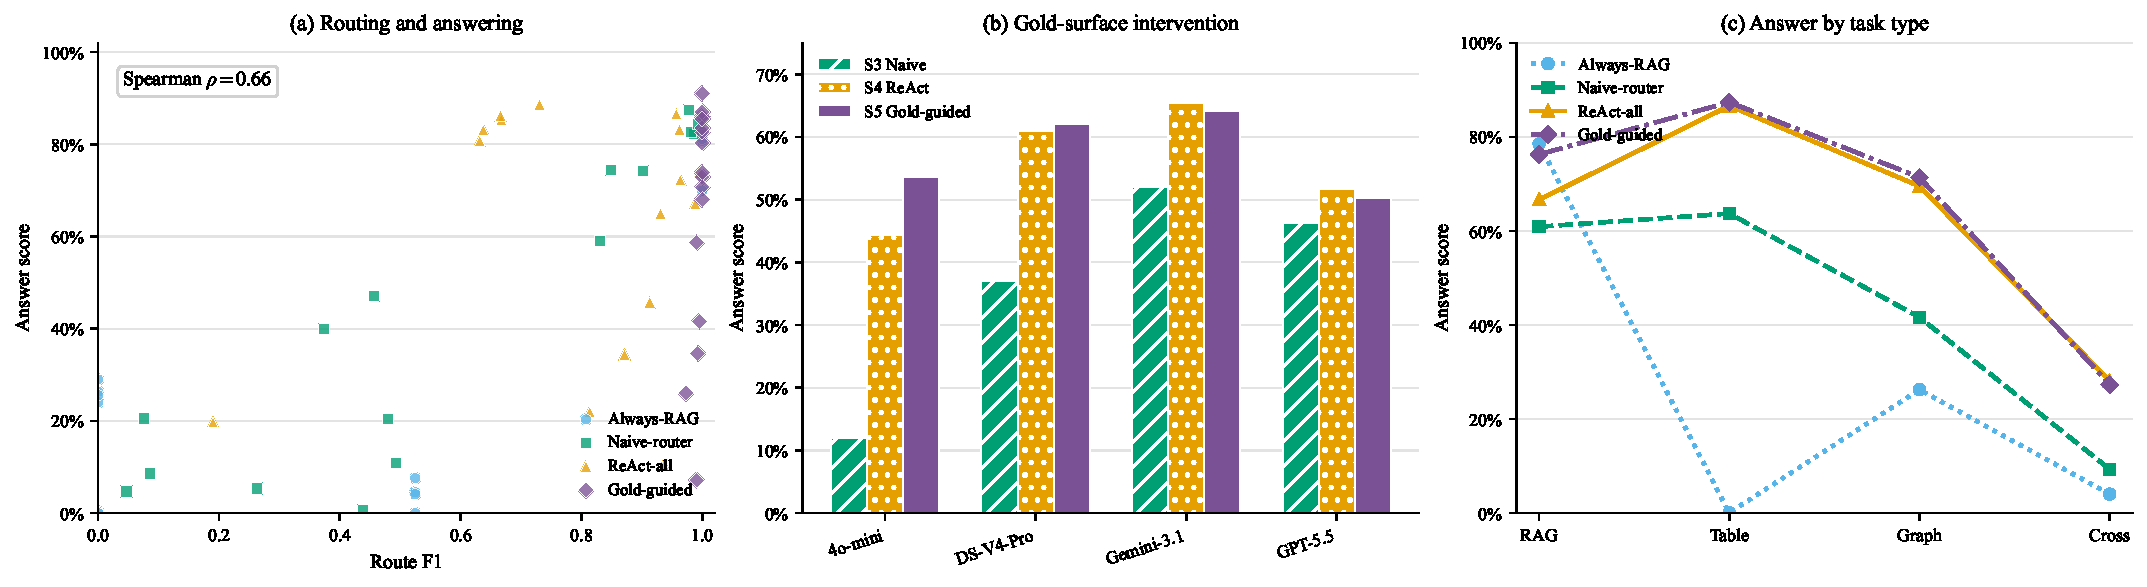
\includegraphics[width=0.98\textwidth]{figure3.pdf}
\caption{Routing and answering exhibit related but distinct behavior.
(a) Route F1 versus Answer across 64 model--setting--task-type buckets
($\rho=0.66$). (b) Answer changes modestly from S4 to the gold-surface
intervention S5. (c) Mean Answer by task type and setting.}
\label{fig:main}
\end{figure*}
\paragraph{Efficiency.}
Let $t_i$ be the observed token count and $b_i$ the task-specific common
budget, fixed at twice the token count of the canonical GPT-4o-mini S5 trace.
The piecewise-linear score is
\[
Q_i=\begin{cases}
1-t_i/(2b_i), & t_i\le b_i,\\
\max\{0,\,1-(t_i-b_i)/b_i\}, & t_i>b_i.
\end{cases}
\]
Thus, $Q_i$ decreases from 1 to 0.5 within budget and reaches 0 at twice the
budget. If no positive budget is available, the implementation assigns the
neutral value $Q_i=1$; this defensive fallback is not triggered by the
released set.

\paragraph{Aggregate.}
The released set has no activated safety-threat annotations, so Safety is
omitted and does not enter this aggregate. We
assign the largest weight to end-task correctness, retain substantial weight
on evidence and routing, and treat efficiency as a secondary objective:
\[
\begin{aligned}
\mathrm{Agg}_i={}&0.35A_i+0.30E_i\\
                 &+0.25F^{\mathrm{route}}_i+0.10Q_i.
\end{aligned}
\]
Equal weighting would assign 25\% to Efficiency and allow a cheap but
incorrect no-tool system to receive substantial credit. The 10\% weight keeps
efficiency consequential without allowing it to dominate task success. We
average $\mathrm{Agg}_i$ across tasks rather than reconstructing it from
rounded column means; component scores remain the primary diagnostic outcomes.

\section{Experiments}
\label{sec:experiments}

\subsection{Experimental Setup}
\label{sec:setup}

\paragraph{Backbones.}
Using identical prompts and tool schemas, we query four proxy-exposed API
identifiers: \texttt{gpt-4o-mini} \citep{openai2024gpt4omini},
\texttt{deepseek-v4-pro} \citep{deepseek2026v4},
\texttt{gemini-3.1-pro-preview} \citep{google2026gemini31pro}, and
\texttt{gpt-5.5} \citep{openai2026gpt55}. Released traces record the requested
identifiers (costs in Appendix~\ref{sec:reproducibility}).

\paragraph{Agent settings.}
Five settings span the routing autonomy spectrum:
(\textbf{S1}) \emph{No-tool} answers from parametric memory only ---
the closed-book baseline;
(\textbf{S2}) \emph{Always-RAG} forces a single \texttt{kb\_search} on every
task;
(\textbf{S3}) \emph{Naive-router} picks exactly one surface up front and
uses only its tools;
(\textbf{S4}) \emph{ReAct-all} exposes all three surfaces and lets the agent
freely interleave them; and
(\textbf{S5}) \emph{Gold-surface guided} is given the required surfaces and
can only use tools within them. This is a guidance intervention rather than a
guaranteed-execution condition: the model must still invoke the relevant
tools, retrieve evidence, and produce the answer. The S4$\to$S5 contrast
estimates the effect of supplying gold surface information.

\paragraph{Tools and inference.}
RAG, Table, and Graph expose search, read-only DuckDB, and graph-traversal
tools, respectively. We use a portable text-based ReAct loop capped at eight
tool turns (median four), with temperature 0 and greedy decoding. Only S4
exposes all three surfaces, creating distractor pressure; S2 and S3 restrict
tool access as defined above. Each task's common Efficiency budget is fixed at
$2\times$ the token count of the canonical GPT-4o-mini S5 trace. Exact setting and tool schemas appear in
Appendix~\ref{sec:agent-details}; implementation and cost details appear in
Appendix~\ref{sec:reproducibility}.

\subsection{Main Results}
\label{sec:mainresults}

% ---- end table_persurface.tex ----
Table~\ref{tab:main} reports every model $\times$ setting on four component
scores and their aggregate. Tool access generally improves Answer over the
no-tool condition, but the gains are non-monotonic across agent settings.
Gemini obtains the highest aggregate under gold guidance (75.7), closely
followed by DeepSeek (74.7), then GPT-4o-mini (71.1) and GPT-5.5 (69.9).
DeepSeek also reaches the second-highest Answer score (62.1) under S5, showing
that its strong result is not driven only by routing or efficiency. All 20
runs contain the same 1{,}151 tasks and retain no protocol-error traces.
Among unconstrained S4 agents, Gemini again leads (73.9 aggregate), followed by
DeepSeek (67.8), GPT-5.5 (66.0), and GPT-4o-mini (57.1). S5 changes the ranking
only slightly but narrows the gap: its aggregate gains over S4 are 14.0 points
for GPT-4o-mini, 6.9 for DeepSeek, 1.8 for Gemini, and 3.9 for GPT-5.5. Thus,
surface guidance helps the weakest router most, while stronger routers derive
less end-to-end benefit from the intervention.

\subsection{Gold Surface Information Improves Routing More Than Answering}
\label{sec:routing-answer}
The S4$\to$S5 contrast in Table~\ref{tab:main} shows that better routing does
not guarantee better answers. Route~F1 rises by 28.3 points for GPT-4o-mini,
20.6 for DeepSeek, 6.3 for Gemini, and 17.2 for GPT-5.5. The corresponding
Answer changes are only $+9.2$, $+1.2$, $-1.3$, and $-1.5$ points. DeepSeek is
particularly diagnostic: near-perfect routing under S5 leaves Evidence
essentially unchanged (77.5 to 77.3) and Answer improves by only 1.2 points.
Gold surface information therefore removes most selection uncertainty without
removing evidence-acquisition, computation, or synthesis errors.
The Evidence changes reinforce this interpretation. From S4 to S5, Evidence
moves by $+6.8$, $-0.2$, $+0.9$, and $-0.8$ points for GPT-4o-mini, DeepSeek,
Gemini, and GPT-5.5, respectively. Except for GPT-4o-mini, constraining the
available surfaces barely changes which gold evidence is recovered. The large
Route gains are therefore not equivalent to large retrieval gains.

\subsection{Performance by Surface Composition}
\label{sec:persurface}
Table~\ref{tab:persurface} and Figure~\ref{fig:main}c decompose Answer by task
type. Single-surface RAG, Table, and Graph peak at 83.6\%, 91.0\%, and 73.9\%,
respectively, whereas cross-surface Answer peaks at only 45.7\%. DeepSeek is
strong on Table under gold guidance (91.0\%) and reaches 34.6\% on cross-surface
tasks, but it still trails Gemini's unconstrained cross-surface result by 11.1
points. The persistent gap across all four backbones indicates that combining
evidence representations, rather than any one surface, is the main challenge.
The single-surface results also reveal different model profiles. GPT-4o-mini's
naive router performs well on Graph (59.0) but poorly on RAG and Table, whereas
DeepSeek, Gemini, and GPT-5.5 exceed 74 on both RAG and Table under S3. Graph
remains less saturated for these three models, and every model loses at least
38 points when moving from its strongest single-surface category to Cross.
This pattern is consistent with a composition bottleneck rather than uniform
task difficulty.

\subsection{Post-Routing Bottlenecks}
\label{sec:failures}
The gap between routing and execution is clearest under S5: all four models
obtain 98.7--99.8 Route~F1, but Evidence remains at 67.1--78.8 and Answer at
50.2--64.1. This pattern is consistent with three failure stages. Low S3 Route
and Evidence indicate selection failures; high Route with incomplete Evidence
under S5 indicates acquisition failures; and residual Answer errors after
strong Evidence indicate computation or synthesis failures. The last stage is most
visible for GPT-5.5, whose S5 cross-surface Answer is only 7.2 despite 99.6
Route~F1, and for DeepSeek, whose near-perfect routing yields only 34.6 on the
same category. Correct surface information is therefore necessary but not
sufficient for composition.
Under S5, the Evidence--Answer gap is 13.5 points for GPT-4o-mini, 15.2 for
DeepSeek, 14.7 for Gemini, and 25.5 for GPT-5.5. Because all four models already
have near-perfect Route scores in this setting, these gaps quantify the loss
that remains after surface selection. GPT-5.5 is the clearest case:
its Evidence score is comparable to the other strong models, but substantially
less of that evidence is converted into a correct final answer.

\subsection{Closed-Book Answerability and Efficiency}
\label{sec:closedbook}
No-tool reaches at most 2.4\% Answer over all 1{,}151 tasks, indicating limited
closed-book answerability but not excluding contamination; we therefore treat
S1 as a diagnostic, not a formal test. Under the common GPT-4o-mini S5 budget
defined in \S\ref{sec:setup}, mean Efficiency is 95.8\% for No-tool, 44.9\% for
ReAct-all, and 54.3\% for Gold-guided. From S4 to S5, it rises by 16.0, 13.4,
4.4, and 3.7 points for GPT-4o-mini, DeepSeek, Gemini, and GPT-5.5. The larger
gains for the first two are consistent with less wasted exploration, while
Answer changes remain small for three models. Efficiency is a normalized, tokenizer-dependent diagnostic weighted
at 10\%; provider-dependent costs are discussed in
Appendix~\ref{sec:reproducibility}.

\section{Conclusion}
\label{sec:conclusion}

WorkSurface-Bench separates routing from answering on 1{,}151 auditable tasks
over documents, tables, and dependency graphs. Across four backbones,
gold-surface guidance raises Route F1 to 98.7--99.8, yet Answer remains at
50.2--64.1. Because S5 supplies required surfaces, it is an intervention
rather than evidence of autonomous routing; its near-perfect Route score helps
localize remaining evidence and computation failures. The decomposed
metrics expose those failures, and cross-surface reasoning remains the central
bottleneck. This distinction suggests that agent evaluations should report
surface selection separately, while system development should target evidence
recovery and cross-surface composition after routing rather than treating
correct routing as sufficient. Future work should broaden workspaces, domains,
and repeated runs.

\clearpage
\section*{Limitations}
The benchmark covers five personas and three knowledge surfaces derived from
Workspace-Bench-Lite, so results may not transfer directly to other enterprise
domains. Automated generation can introduce templated language, so we built a
2{,}000-item candidate pool and retained 1{,}151 items passing strict checks by
at least two of three model auditors. Three annotators independently audited
200 stratified items; all 200 pass all six dimensions by majority vote, but a
sample cannot prove that every item is flawless. Persona and
source-task frequencies remain uneven. Efficiency uses a fixed GPT-4o-mini
reference trace and should be interpreted as a secondary, tokenizer-dependent
diagnostic. Broader domains and repeated runs are left to future work.

\section*{Ethics Statement}
The benchmark contains no personal data and uses public or grounded synthetic
artifacts inherited from Workspace-Bench; the released source lock supports
provenance auditing.

\bibliography{custom}

\appendix
\section{Quality Audits and Construction Details}
\label{sec:appendix}

\subsection{Rubric-to-Task Conversion}
The 100 source tasks carry 1{,}850 rubrics across four Workspace-Bench rubric
types (Basic Evaluation: 450, Outcome Evaluation: 1{,}030, Process Evaluation:
339, Result Evaluation: 31). Deterministic and proof-carrying generators first
produce a 2{,}000-item candidate pool. GPT-5.5 retains 1{,}465 items passing
answerability, gold correctness, naturalness, atomicity, and leakage checks;
independent DeepSeek and Gemini audits then yield 1{,}151 items passing the
strict criteria under at least two of three models.

\subsection{Surface Coverage Validation}
Each routable surface must support executable gold construction and a
non-trivial task set. The final release contains 453 table-bearing items with
reproducible DuckDB results, 601 RAG-bearing items with verified source spans,
and 600 graph-bearing items whose dependency paths match source annotations.
All five personas and all three surfaces remain represented after screening.

\subsection{Gold-Answer Audit}
Because we never take a gold answer from LLM free text, we can \emph{execute}
or \emph{re-verify} every gold value directly. We audited the whole set:
\textbf{(i)} all 453 table-bearing items have queries that execute against the
DuckDB registry and reproduce their gold results; \textbf{(ii)} all 601
RAG-bearing items have an exact evidence span; and \textbf{(iii)} all 600
graph-bearing items have valid nodes, paths, or complete neighbor sets.
This audit is fully automated and re-runnable from the released code.

\subsection{Independent Human Audit}
Three annotators independently reviewed the same stratified 200-item sample:
30 Graph, 40 Table, 30 RAG, 25 Graph+Table, 35 RAG+Graph, 25 RAG+Table, and all
15 three-surface tasks. By majority vote, all 200 items are natural,
answerable, dependent on every annotated surface, gold-correct, atomic and
unambiguous, and free of a leakage cue. Required-surface necessity and
atomicity are unanimous on 200/200 items; 192/200 items are unanimous across
all six dimensions. Pairwise agreement ranges from 98.7\% (naturalness) to
100\% (surface necessity and atomicity).

\subsection{Distribution}
\label{sec:distribution}
Figure~\ref{fig:distribution} shows the benchmark's cross-cutting
distributions. Cross-surface is the largest class (42\%), followed by Table
(24\%), RAG (19\%), and Graph (15\%); personas span five roles with the operational two dominating,
reflecting the Workspace-Bench-Lite source; answer types cover number, list,
and string. Derivation paths are intentionally uneven: filtering retains every
strictly verified item rather than enforcing equal quotas, while no single
path accounts for a majority of the release.

\begin{figure*}[t]
\centering
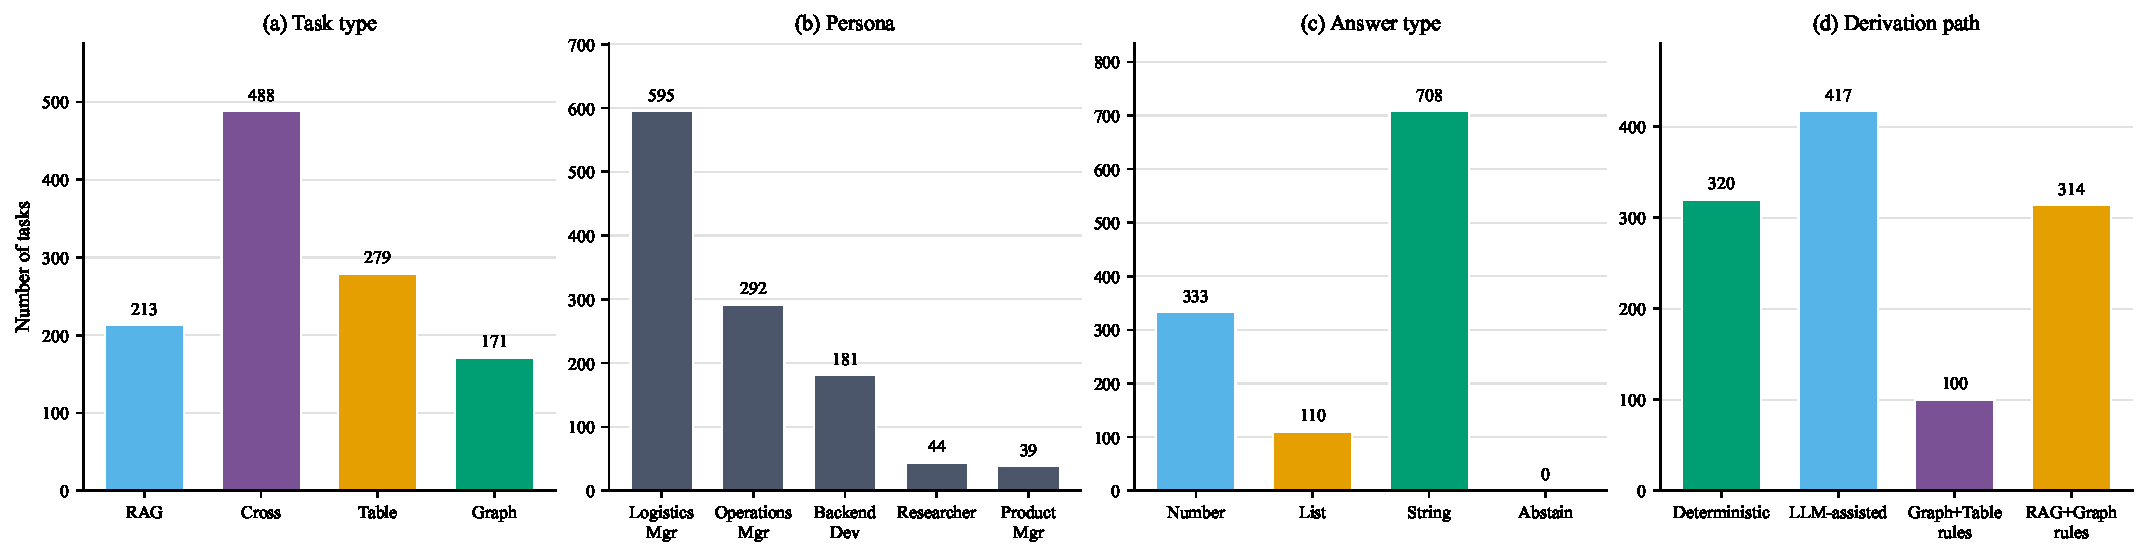
\includegraphics[width=0.98\textwidth]{figure4_distribution.pdf}
\caption{Dataset distributions across (a) task type, (b) persona, (c) answer
type, and (d) derivation path. Frequencies are intentionally non-uniform:
filtering prioritizes verifiability and strict surface necessity over quotas.}
\label{fig:distribution}
\end{figure*}

\subsection{Closed-Book Answerability Diagnostic}
\label{sec:appendix-closedbook}
The S1 no-tool setting reaches at most 2.4\% Answer over all 1{,}151 tasks. This
result indicates limited closed-book answerability, but it is not a formal
contamination test and does not rule out item-level memorization.

\subsection{Task Examples}
Two illustrative items (abbreviated for space):
\smallskip
\noindent\textbf{cross\_surface (LLM-assisted, gold via query execution).}
\emph{Question}: ``For workspace task 107: what is the total sales amount
across the Asia Pacific region?''
\emph{Gold}: \texttt{800511.75} (number).
\emph{Gold evidence}: [surface=rag, file=\texttt{t107\_\_report.md},
span=``Asia Pacific''; surface=table, table=\texttt{t107\_\_asia\_pacific\_orders},
query=\texttt{SELECT ROUND(SUM(sales),2) FROM ...}].
\emph{Required surfaces}: \{rag, table\}.

\section{Agent Configuration Details}
\label{sec:agent-details}

Table~\ref{tab:agent-settings} gives the executable distinction among the five
settings. S5 receives only the names of the required surfaces: it is not given
the gold query, evidence, tool sequence, or answer. Route scores are computed
from surfaces actually used in the trace, which is why S5 Route-F1 need not be
100\%.

\begin{table*}[t]
\centering\small
\setlength{\tabcolsep}{3.5pt}
\begin{tabular*}{\textwidth}{@{\extracolsep{\fill}}p{0.10\textwidth}p{0.15\textwidth}p{0.15\textwidth}p{0.21\textwidth}p{0.27\textwidth}}
\toprule
\textbf{Setting} & \textbf{Exposed surfaces} & \textbf{Initial behavior} & \textbf{Subsequent interaction} & \textbf{Purpose} \\
\midrule
S1 No-tool & None & Answer directly & No tools & Closed-book answerability baseline \\
S2 Always-RAG & RAG only & Forced \texttt{kb\_search} & One-shot answer from returned snippets & Fixed single-surface baseline \\
S3 Naive-router & One selected surface & Choose exactly one of RAG/Table/Graph & ReAct restricted to that surface & One-shot surface routing \\
S4 ReAct-all & RAG, Table, Graph & No forced call & Dynamically interleave exposed tools, up to 8 turns & Unconstrained agent under distractor pressure \\
S5 Gold-guided & Required surfaces only & No forced call & Dynamically interleave tools within the required set, up to 8 turns & Surface-information intervention \\
\bottomrule
\end{tabular*}
\caption{Operational definitions of the five agent settings. All settings use
the same question and answer format; only tool exposure and the forced initial
behavior differ.}
\label{tab:agent-settings}
\end{table*}

For S3--S5, each ReAct turn emits exactly one JSON object containing either a
tool call or \texttt{final\_answer}. RAG exposes \texttt{kb\_search}; Table
exposes \texttt{table\_list}, \texttt{table\_describe}, and read-only
\texttt{table\_query}; Graph exposes entity search, neighbor lookup, and
traversal. Invalid JSON receives a format-repair prompt but still consumes a
turn. Runs use greedy decoding at temperature 0 and terminate on a final
answer or after eight tool turns.

\section{Reproducibility, Cost, and Access}
\label{sec:reproducibility}

\paragraph{Software.}
We release, under an open-source license, (i) the source-download and
freeze scripts (Workspace-Bench-Lite commit hash + per-file SHA-256), (ii) the
surface-projection and SOP-metadata converters, (iii) the deterministic and LLM-assisted task
derivers with a shared verifiable-gold contract, (iv) the scoring package with
nine unit tests, and (v) the agent harness (portable text-based ReAct loop,
per-task backbone, task-level checkpointing).

\paragraph{Runs.}
Main experimental numbers come from one canonical trajectory per
(task, model, setting) through an OpenAI-compatible proxy. The initial sweep
used moderate concurrency; failed trajectories were retried at lower
concurrency, with successful retries replacing failed rows. The final release
contains 23{,}020 retained traces with no protocol errors for \texttt{gpt-4o-mini},
\texttt{deepseek-v4-pro}, \texttt{gemini-3.1-pro-preview}, and
\texttt{gpt-5.5}.

\paragraph{Cost.}
Exact monetary cost depends on the proxy and model pricing in effect at run
time. We therefore release per-trajectory token counts, retry status, and the
aggregation scripts, allowing costs to be recomputed under any provider's
pricing schedule.

\paragraph{License and access.}
The derived benchmark inherits Workspace-Bench-Lite's license (see the
source repository). Our derived artifacts (task JSONL, canonical KB text,
DuckDB parquet registry, surface graphs, scoring code, and agent harness) are
released under CC~BY~4.0 for data and Apache~2.0 for code. The
\texttt{wsb\_lock.json} freezes the source commit and per-file SHA-256 so any
future re-derivation is bit-reproducible.

\section{Datasheet}
\label{sec:datasheet}

We include an abbreviated Datasheet for Datasets~\cite{gebru2018datasheets}.

\paragraph{Motivation.}
WorkSurface-Bench was created to evaluate whether enterprise agents can
\emph{route} across heterogeneous knowledge surfaces (documents, tables,
dependency graphs), separately from answer correctness. Among the surveyed
benchmarks, none reports routing over these three workspace representations as
a separate metric.

\paragraph{Composition.}
Each instance is an atomic question over one persona-scoped workspace, with a
gold answer, required surfaces, expected tool types, and evidence annotations.
1{,}151 instances total; see Table~\ref{tab:stats} and
Figure~\ref{fig:distribution} for distributions.

\paragraph{Collection process.}
Instances are derived automatically from Workspace-Bench-Lite (English split,
commit \texttt{60b08b1c}) via the pipeline in \S\ref{sec:dataset}. Three
human annotators independently audited a stratified 200-item sample; the
underlying WSB source inherits its authors' expert validation.

\paragraph{Preprocessing.}
Documents are rendered to canonical UTF-8 markdown; tables are normalized and
loaded into a per-workbook DuckDB view registry with provenance columns; the
dependency graph is enriched with programmatic edges. The raw source is
retained (frozen by hash), so preprocessing is fully reversible.

\paragraph{Uses.}
Intended: benchmarking enterprise routing agents, ablations over surface
selection, calibration studies (abstain), reproducibility research.
Not intended: training data (the set is small and constructed from
mixed-provenance content), safety-critical decisions, or production
deployment gates.

\paragraph{Distribution and maintenance.}
The versioned dataset and code are hosted at the repository linked in the
abstract; issues accept fixes and error reports. Future releases will improve
abstain balance, persona coverage, and held-out evaluation.

\paragraph{Ethics and privacy.}
The dataset contains no personally identifying or human-subject data. Files
are public resources or grounded synthetic artifacts inherited from
Workspace-Bench-Lite. Because some source content is LLM-generated,
memorization is possible; the closed-book diagnostic characterizes
answerability without claiming to rule out contamination.

\paragraph{Broader impact.}
The benchmark helps deployers test whether agents follow the right retrieval
path. Its main risk is over-generalization: scores on scenario-grounded hybrid
data should not serve as deployment gates without target-system evaluation.

\end{document}
